% vorlesung 28, 10.02.2011 (Fr.) (Claudia Dieckmann)
\chapter{Approximationsalgorithmen}
\section{Entscheidungs- und Optimierungsprobleme}
Bisher haben wir Komplexitätsklassen wie \textsf{P}, \textsf{NP} oder \textsf{PSpace} betrachtet. Dabei handelte es sich immer um \textit{Entscheidungsprobleme}. Entscheidungsprobleme sind Probleme, auf die eine Antwort immer "`Ja"' oder "`Nein"' ($0$ oder $1$) ist. Es gibt jedoch viele Probleme, bei denen es mehrere gültige Lösungen gibt und die "`beste"' Lösung gesucht wird. Solche Probleme nennt man \textit{Optimierungsprobleme}. Soll die gesuchte "`beste"' Lösung möglichst groß sein, spricht man von einem \textit{Maximierungsproblem}, soll die Lösung möglichst klein sein von einem \textit{Minimierungsproblem}.

Den meisten Optimierungsproblemen können wir ein Entscheidungsproblem zuordnen und den meisten Entscheidungsproblemen ein Optimierungsproblem. Es gibt also eine Art Beziehung zwischen einzelnen Entscheidungs- und einzelnen Optimierungsproblemen.

Betrachten wir als Beispiel das Problem des Handlungsreisenden \textsc{TSP} (\textit{travelling salesman problem}). Gegeben ist ein gerichteter vollständiger Graph $G=(V, E)$ und eine Zahl $k \in \mathbb{N}$. Gefragt ist, ob es eine Rundreise der Länge $k$ gibt. Das zuständige Optimierungsproblem versucht die kürzeste Rundreise zu finden.

\begin{Def}
  \hspace{\parindent}Ein Optimierungsproblem heißt \textit{\textsf{NP}-schwer}, wenn das zugehörige Entscheidungsproblem \textsf{NP}-schwer ist.
\end{Def}

\begin{Anm}
  \hspace{\parindent}\textsf{NP} ist eine Klasse von Entscheidungsproblemen, daher werden Optimierungsprobleme nicht als \textsf{NP}-vollständig bezeichnet.
\end{Anm}

\begin{Def}[optimale Lösung]
  \hspace{\parindent}Sei $P$ ein Optimierungsproblem mit Kostenfunktion $c$. Sei $I$ eine Eingabe für $P$. Die Lösung $f_{opt}(I)$ heißt \textit{optimal}, falls $c(f_{opt}(I)) \le c(f(I))$ für jede andere Lösung $f$ gilt und $P$ ein Minimierungsproblem ist. Ist $P$ ein Maximierungsproblem, so heißt $f_{opt}(I)$ \textit{optimal}, falls $c(f_{opt}(I)) \ge c(f(I))$ für jede andere Lösung $f$ gilt.
\end{Def}

\begin{Def}[$\alpha$-approximativ]
  \hspace{\parindent}Ein Algorithmus $A$ heißt \textit{$\alpha$-approximativ} (mit $\alpha \in \mathbb{R}$) für ein Optimierungsproblem $P$ genau dann, wenn er eine Lösung $f_A$ für $P$ liefert mit $c(f_A(I)) \le \alpha \cdot c(f_{opt}(I))$ bei Minimierungsproblemen und
  $c(f_A(I)) \ge \alpha \cdot c(f_{opt}(I))$ bei Maximierungsproblemen.
\end{Def}

\section{Beispiele für Approximationsalgorithmen}
Wir wollen ein paar beispielhafte Approximationsalgorithmen betrachten. Auch wenn die Entscheidungsprobleme, die wir den jeweiligen Optimierungsproblemen zuordnen können, aus den vorhergehenden Kapiteln bekannt sein sollten, werden wir sie jeweils nochmals kurz vorstellen.

\subsection{Vertex-Cover (Überdeckende Knotenmenge)}
Beim Entscheidungsproblem \textsc{VC} ist ein ungerichteter Graph $G=(V,E)$ und eine Zahl $k \in \mathbb{N}$ gegeben. Das Problem stellt folgende Frage: gibt es eine Teilmenge der Knoten $U \subset V$ der Größe $k$, so dass für alle $\{u, v \} \in E$ entweder $u \in U$ oder $v \in U$ gilt?

Dazu können wir folgendes Optimierungsproblem formulieren: Finde eine überdeckende Knotenmenge minimaler Größe in einem ungerichteten Graphen $G=(V,E)$. Zur Lösung wollen wir einen Approximationsalgorithmus vorstellen, der als Eingabe einen ungerichteten Graphen $G=(V,E)$ bekommt.

\begin{Alg}[Approximationsalgorithmus für Vertex Cover]
  \begin{algorithmic}[1]
    \State $U = \emptyset$
    \While{$E \ne \emptyset$}
      \State Nimm beliebige Kante $e=\{u, v\} \in E$ und füge $u$ und $v$ zu $U$ hinzu.
      \State Entferne alle Kanten aus $E$, die entweder zu $u$ oder zu $v$ inzident sind.
    \EndWhile
  \end{algorithmic}
\end{Alg}

%Approximationsalgorithmus für Vertex Cover.
%Eingabe: $G=(V,E)$\\
%1. $U = \emptyset$\\
%2. Nimm beliebige Kante $e=\{u, v \} \in E$ und füge $u$ und $v$ zu $U$ hinzu.\\
%3. Entferne alle Kanten aus $E$, die entweder zu $u$ oder zu $v$ inzident sind.\\
%4. Wiederhole von Zeile 2 an, bis $E = \emptyset$.

Die Laufzeit dieses Approximationsalgorithmus liegt in $\mathcal{O}(|E| + |V|)$. Wir wollen verdeutlichen, dass der Algorithmus korrekt arbeitet: Eine Kante $e = \{ u, v \} \in E$ wird nur dann aus $E$ entfernt (Zeile 4), wenn entweder $u \in U$ oder $v \in U$. Da zum Schluss $E = \emptyset$, ist jede Kante aus $E$ entfernt worden und somit überdeckt. Abbildung \vref{kap7VCBsp} zeigt ein Beispiel.

\begin{figure}[htb]
  \centering
  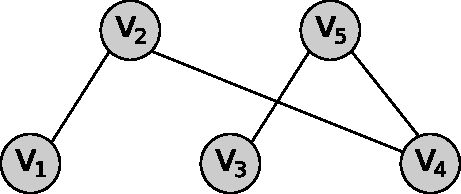
\includegraphics[scale=.66]{kap7VCBsp}
  \caption{Der Approximationsalgorithmus könnte auf diesem Graphen zum Beispiel erst die Kante $\{v_4, v_5\}$ auswählen. Dann wäre $U=\{v_4, v_5\}$ und $E=\{\{v_1, v_2\}\}$. Als VC würde der Algorithmus dann $U=\{v_4, v_5, v_1, v_2\}$ finden. Die optimale überdeckende Knotenmenge ist $U_{opt} = \{ v_2, v_5 \}$. Es gilt hier offensichtlich $|U| = 2 \cdot |U_{opt}|$.}
  \label{kap7VCBsp}
\end{figure}

\begin{Satz}
  \hspace{\parindent}Dieser Algorithmus ist $2$-approximativ.
\end{Satz}

\begin{Bew}
  \hspace{\parindent}Zu zeigen ist $c(f_A(I)) \le 2 \cdot c(f_{opt}(I))$ gilt. $I$ ist dabei die Eingabe, hier also ein ungerichteter Graph $G=(V,E)$. $f_A(I)$ ist die vom Algorithmus konstruierte überdeckende Knotenmenge ($U$ nach Ende des Algorithmus). $f_{opt}(I)$ ergibt die optimale überdeckende Knotenmenge $U_{opt}$. Wir müssen also $|U| \le 2 \cdot |U_{opt}|$ zeigen.
  
  Sei $p$ die Anzahl der Schleifendurchläufe. $p$ entspricht also der Anzahl der Kanten, die ausgewählt werden. Seien $e_1 = \{ u_1, v_1 \}$ und $e_2 = \{u_2, v_2\}$ zwei ausgewählte Kanten, dann ist $u_1 \neq u_2$, $u_1 \neq v_2$, $v_1 \neq u_2$ und $v_1 \neq v_2$. Jede überdeckende Knotenmenge enthält also mindestens $p$ Knoten, woraus folgt $U_{opt} \ge p$. Da in jedem Schleifendurchlauf genau zwei Knoten zu $U$ hinzugefügt werden, ist $|U| = 2 \cdot p$. Daher: $|U| = 2 \cdot p \le 2 \cdot |U_{opt}|$.
\end{Bew}

\subsection{Approximationsalgorithmus für TSP}
Schränkt man das Problem des Handlungsreisenden (\textsc{TSP}, \textit{travelling salesman problem}) ein wenig ein, so lässt sich ein Approximationsalgorithmus finden. \textsc{$\varDelta$-TSP} ist ein Entscheidungsproblem, eine Variante von \textsc{TSP}. Als Eingabe dient eine $n \times n$ Abstandsmatrix $D$ mit $n=|V|$ und eine Zahl $k \in \mathbb{N}$. Die Einschränkung im Vergleich zum allgemeinen TSP ist: $D$ erfüllt die Dreiecksungleichung $d_{ij} + d_{jk} \ge d_{ik}$. Das Entscheidungsproblem fragt, ob es eine Tour der Länge $\le k$ gibt. \textsc{$\varDelta$-TSP} ist \textsf{NP}-vollständig. Man kann zeigen, dass $\mathsc{HC} \le_p \operatorname{\varDelta-\mathsc{TSP}}$. Das Optimierungsproblem \textsc{$\varDelta$-TSP} sucht die kürzeste Tour.

Bevor wir einen Approximationsalgorithmus für \textsc{$\varDelta$-TSP} besprechen führen wir Multigraphen und Eulerwege ein:

\begin{Def}[Multigraph]
  \hspace{\parindent}Ein \textit{Multigraph} $M=(V,E)$ ist ein Graph, bei dem zwischen zwei Knoten mehr als eine Kante existieren darf.
\end{Def}

\begin{figure}[htb]
  \centering
  \includegraphics{kap7Multigraph}
  \caption{Ein Multigraph}
  \label{kap7Multigraph}
\end{figure}

\begin{Def}[eulerscher Graph, Eulerweg]
  \hspace{\parindent}$G$ heißt \textit{eulersch} genau dann, wenn ein geschlossener Weg existiert, der jeden Knoten mindestens einmal und jede Kante genau einmal enthält. Dieser Weg heißt \textit{Eulerweg}.
\end{Def}

\begin{Satz}
  \hspace{\parindent}$G$ ist eulersch genau dann, wenn $G$ zusammenhängend ist und jeder Knoten geraden Grad hat.
\end{Satz}

Den Satz präsentieren wir hier ohne Beweis. Ein Eulerweg kann in $\mathcal{O}(|V| + |E|)$ bestimmt werden.

Zur Lösung des Optimierungsproblems \textsc{$\varDelta$-TSP} wollen wir eine Heuristik nutzen: die Baumheuristik für \textsc{$\varDelta$-TSP}. Die Eingabe für \textsc{$\varDelta$-TSP} ist ein vollständiger Graph $G=(V,E)$, gegeben durch die Abstandsmatrix $D$, die die Dreiecksungleichung erfüllt.

\begin{Alg}[Baumheuristik für $\varDelta$-TSP]
  \begin{algorithmic}[1]
    \State berechne MST $T$ von $G$
    \State Verdopple jede Kante in $T$, $T$ wird also zum Multigraph $M$
    \State Bestimme Eulerweg $w$ in $M$, o.B.d.A. gilt $w = i_1, \ldots, i_2, \ldots, i_3, \ldots, i_n$
    \State Bestimme Tour $\tau$ aus $w$, indem immer nur das erste Vorkommen des Knotens $i$ beachtet wird
  \end{algorithmic}
\end{Alg}
%Eingabe $G=(V, E)$ gegeben durch Abstandsmatrix $D$.\\
%1. berechne MST $T$ von $G$.\\
%2. Verdopple jede Kante in $T \rightarrow$ Multigraph $M$.\\
%3. Bestimme Eulerweg $w$ in $M$. $w = i_1, \ldots, i_2, \ldots, i_3, \ldots, i_n$\\
%   Bestimme Tour $\tau$ aus $w$, in dem immer nur das erste Vorkommen von Knoten $i$ betrachtet wird.

\begin{Bsp}
  \hspace{\parindent}Wir wollen die Baumheuristik an einem Beispiel nachvollziehen. In Abbildung \vref{kap7Baumheuristik} sind ein Graph, der zugehörige MST und der entsprechende Multigraph abgebildet. Im Multigraph $M$ können wir folgenden Eulerweg finden: $v_1, v_3, v_2, v_3, v_4, v_3, v_1$. Daraus ergibt sich folgende Tour: $v_1, v_3, v_2, v_4, (v_1)$.
  
  \begin{figure}[htb]
    \centering
    \subfloat[Der Graph $G$\label{kap7BaumheuristikG}]%
      {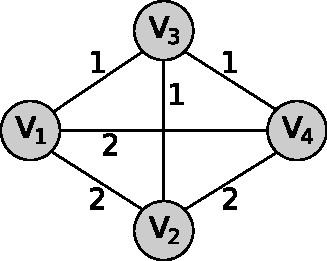
\includegraphics[width=.29\textwidth]{kap7BaumheuristikG}}\hspace{.05\textwidth}
    \subfloat[Der zugehörige MST $T$\label{kap7BaumheuristikMST}]%
      {\includegraphics[width=.29\textwidth]{kap7BaumheuristikMST}}\hspace{.05\textwidth}
    \subfloat[Der konstruierte Multigraph $M$\label{kap7BaumheuristikMG}]%
      {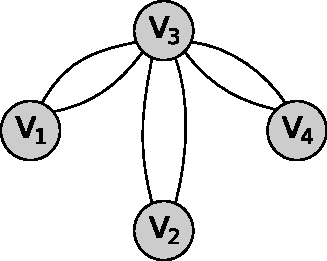
\includegraphics[width=.29\textwidth]{kap7BaumheuristikMG}}
    \caption{Ein Beispiel für die Baumheuristik. \subref{kap7BaumheuristikG} zeigt einen Graphen, an dem wir die Baumheuristik beispielhaft nachvollziehen wollen. Der zugehörige MST ist in \subref{kap7BaumheuristikMST} zu sehen, der Multigraph in \subref{kap7BaumheuristikMG}.}
    \label{kap7Baumheuristik}
  \end{figure}
\end{Bsp}

\begin{Lma}
  \hspace{\parindent}Sei $M$ ein eulerscher Multigraph auf der Knotenmenge $V= \{ 1, \ldots, n\}$ mit Kosten $c(M) = \sum_{(i,j) \in E_M} d_{ij}$. Dann lässt sich eine Rundreise $\tau$ auf den Knoten $V$ in Zeit $\mathcal{O}(|E|)$ finden mit $c(\tau) \le c(M)$.
\end{Lma}

\begin{Bew}
  \hspace{\parindent}Sei $w$ Eulerweg in $M$:
  \[ w = i_1 \underbrace{\ldots}_{\alpha_1} i_2 \underbrace{\ldots}_{\alpha_2} i_3 \ldots i_n \underbrace{\ldots}_{\alpha_n} \]
  $i_j$ sind Knoten, die vorher nicht in $w$ vorkamen. $\alpha_j$ ist der Weg von $i_j$ nach $i_{j+1}$, der nur Knoten aus $\{i_1, \ldots, i_j\}$ enthält. Aus der Definition eines Eulerwegs folgt $c(w) = c(M)$. Betrachte Tour $\tau = i_1, i_2, \ldots, i_n$. Dann gilt:
    \[ c(\tau) = \sum_{j=1}^{n-1} d_{i_j i_{j+1}} + d_{i_n i_1}\]
  Wegen der Dreiecksungleichung ist $d_{i_j i_{j+1}} \le c(\alpha_j)$. Damit gilt:
    \[ c(\tau) = \sum_{j=1}^{n-1} d_{i_j i_{j+1}} + d_{i_n i_1} \le c(\alpha_1) + c(\alpha_2) + \ldots + c(\alpha_n) = c(w)\]
  Es gilt also $c(\tau) \le c(w) = c(M)$.
\end{Bew}

Der Eulerweg lässt sich in $\mathcal{O}(|E| + |V|)$ finden, die Tour daher auch.

\begin{Satz}
  \hspace{\parindent}Die Baumheuristik für $\varDelta$-TSP ist $2$-approximativ.
\end{Satz}

\begin{Bew}
  \hspace{\parindent}Die optimale Tour $\tau_{opt}$ enthält einen aufspannenden Baum $T'$. Es folgt $c(\tau_{opt}) \ge c(T')$. Sei $T$ ein minimal aufspannender Baum für den selben Graphen. Dann muss $c(T') \ge c(T)$ gelten, sonst wäre $T$ nicht minimal. Gemäß der Konstruktion von $M$ ist $c(M) = 2 \cdot c(T)$. Für die durch die Baumheuristik konstruierte Tour $\tau$ gilt nach dem Lemma $c(\tau) \le c(M)$. Daraus folgt $c(\tau) \le c(M) \le 2 \cdot c(T) \le 2 \cdot c(\tau_{opt})$.
\end{Bew}

\begin{figure}[htb]
  \centering
  \subfloat[\label{kap7DeltaTSPMST}]{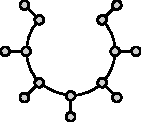
\includegraphics{kap7DeltaTSPMST}}\hspace{2em}
  \subfloat[\label{kap7DeltaTSPMG}]{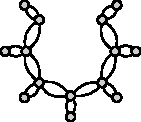
\includegraphics{kap7DeltaTSPMG}}\hspace{2em}
  \subfloat[\label{kap7DeltaTSPLsg}]{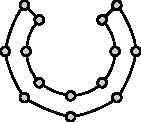
\includegraphics{kap7DeltaTSPLsg}}\hspace{2em}
  \subfloat[\label{kap7DeltaTSPOpt}]{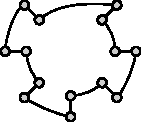
\includegraphics{kap7DeltaTSPOpt}}
  \caption{Bei TSP geht man meistens von einem vollständigen Graphen aus. Betrachten wir hier ein Beispiel für \textsc{$\varDelta$-TSP} in einem Graphen mit $14$ Knoten. \subref{kap7DeltaTSPMST} zeigt einen möglichen Spannbaum, \subref{kap7DeltaTSPMG} den entsprechenden Multigraph mit leicht zu findender Euler-Tour, \subref{kap7DeltaTSPLsg} eine durch die Baumheuristik gefundene Lösung, die quasi zwei Kreise umfasst und \subref{kap7DeltaTSPOpt} eine optimale Lösung, die einen Kreis beinhaltet. Natürlich arbeitet die Baumheuristik auch hier $2$"=approximativ.}
  \label{kap7DeltaTSP}
\end{figure}

Abbildung \ref{kap7DeltaTSP} zeigt ein weiteres Beispiel, \ref{kap7DeltaTSPLsg} ist eine mittels Baumheuristik gefundene Lösung, \ref{kap7DeltaTSPOpt} eine optimale Lösung. Erstere umfasst augenscheinlich zwei Kreise, letztere einen Kreis. Die Anzahl der genutzten Kanten ist jedoch identisch.


% Vorlesung 29, 14.02.2011 (Mo.) Alt
%$\varDelta$-TSP ist TSP mit Dreiecksungleichung
%Das zugehörige Entscheidungsproblem ist \textsf{NP}-schwer. Die "`Baumheuristik"' liefert 2-Approx

% Beispiel
%Abbildung 29-1

%Abstand zwischen zwei Punkten $L_{\infty}$-Metrik: \[ d_{\infty}((x_1, y_2), (x_2, y_2)) = max(|x_1 - x_2|, |y_1 - y_2|) \] Man nimmt den Maximalen unterschied zwischen den x und y werten. Z.B. $d_{\infty}(p_1, p_2) = 1$ $d_{\infty}(p_6, p_7) = 3$. Ist eine Metrik, halt eine andere als die meistens genutzte Euklidische.

%Die Baumheuristik ist 2-approximativ. Kann man das noch verbessern?

\subsection{Heuristik von Christofides}
Die Frage, die sich bei einem $\alpha$"=approximativen Algorithmus offensichtlich stellt lautet: kann man das noch verbessern? Im Fall von \textsc{$\varDelta$-TSP} können wir es verbessern.

Betrachten wir ein neues Beispiel. Auch hier gehen wir wieder von einem vollständigen Graphen aus, diesmal mit 8 Knoten. In Abbildung \vref{kap7Christofides1} sehen wir die Knoten des Graphen und ein dahinter liegendes Gitter, dass uns helfen soll den Abstand zwischen den Knoten zu bestimmen. Dazu nutzen wir jedoch nicht die euklidische Metrik, sondern die $L_{\infty}$-Metrik. Den Abstand zwischen zwei Punkten berechnen wir als den maximalen Unterschied zwischen den X- und den Y-Werten beider Punkte, also: $d_{\infty}((x_1, y_1), (x_2, y_2)) = max(|x_1 - x_2|, |y_1 - y_2|)$.

\begin{figure}[htb]
  \centering
  \includegraphics{kap7Christofides1}
  \caption{Im Beispiel gehen wir von einem vollständigen Graphen mit acht Knoten aus. Die Abbildung verdeutlicht die Lage der Knoten zueinander, das Gitter dient zur Berechnung ihres Abstands.}
  \label{kap7Christofides1}
\end{figure}

Auf das Handschlaglemma wollen wir hier nicht näher eingehen. Für uns ist jetzt nur wichtig zu wissen, dass sich aus diesem Lemma ergibt, dass jeder Graph eine gerade Zahl Knoten ungeraden Grads hat.

Wir konstruieren den MST $T$ wie gehabt und betrachten die Knoten ungeraden Grads. Wie gesagt ist das eine gerade Anzahl von Knoten. Darauf konstruieren wir ein perfektes Matching $M$ minimalen Gewichts (\textit{minimum perfect matching}), also ein Matching, bei dem jeder der betrachteten Knoten zu einer Kante des Matchings inzident ist. Das ist möglich in polynomieller Laufzeit, zum Beispiel mit dem Algorithmus von Lawler, der in $\mathcal{O}(n^2)$ arbeitet. Nun betrachten wir den Graphen $G'=(V, T \cup M)$. Kanten, die im  minimalen Spannbaum $T$ und im Matching $m$ vorkommen, sind in $G'$ als Doppelkante enthalten. $G'$ ist also ein Multigraph. Dieser Graph ist eulersch, denn jeder Knoten hat geraden Grad. Auf diesem Graphen konstruieren wir eine Eulertour und fahren fort, wie zuvor bei der Baumheuristik.

Abbildung \vref{kap7ChristofidesMST} zeigt den minimalen Spannbaum unseres Beispiels, \ref{kap7ChristofidesMG} den eulerschen Multigraphen, in dem die Kanten des Spannbaums und des Matchings vereint wurden.

\begin{figure}[htb]
  \centering
  \subfloat[\label{kap7ChristofidesMST}]{\includegraphics{kap7ChristofidesMST}}\hspace{2em}
  \subfloat[\label{kap7ChristofidesMG}]{\includegraphics{kap7ChristofidesMG}}\hspace{2em}
  \caption{\subref{kap7ChristofidesMST} zeigt den minimalen Spannbaum (MST) zum Graph aus Abbildung \vref{kap7Christofides1}. \subref{kap7ChristofidesMG} zeigt den Graph, in dem die Kanten des Matchings und des MSTs bereits vereint sind.}
  \label{kap7ChristofidesMSTMG}
\end{figure}

Die Eulertour im Graph aus Abbildung \vref{kap7ChristofidesMG} ist: $1, 2, 7, 8, 7, 5, 6, 5, 4, 3, 1$. Die mit der Christofides-Heuristik gefundene Tour ist dann: $1, 2, 7, 8, 5, 6, 4, 3$ und hat Kosten in Höhe von $15$ (nach der $L_{\infty}$"=Metrik). Die optimale Tour hat $14$ Kosten und ist in Abbildung \vref{kap7ChristofidesOpt} zu sehen.

\begin{figure}[htb]
  \centering
  \includegraphics{kap7ChristofidesOpt}
  \caption{Zu sehen ist die optimale Tour zum Beispiel aus Abbildung \ref{kap7Christofides1}.}
  \label{kap7ChristofidesOpt}
\end{figure}

\begin{Satz}
  \hspace{\parindent}Die Heuristik von Christofides ist ein $\frac{3}{2}$-approximativer Algorithmus für $\varDelta$-TSP.
\end{Satz}

\begin{Bew}
  \hspace{\parindent}Aus der Dreiecksungleichung ergibt sich $c(\tau) \le c(G')$. Für die konstruierte Rundreise $\tau$ gilt daher:
  \[ c(\tau) \le c(G) = c(T) + c(M) \]
  
  Betrachte $\tau_{opt} = \alpha_1 i_1 \alpha_2 i_2 \ldots i_{2m} \alpha_{2m+1}$. $i_j$ sind die Knoten, die in $T$ ungeraden Grad haben, $\alpha_k$ sind die Teilsequenzen dazwischen. Abbildung \ref{kap7ChristofidesBew} veranschaulicht das.
  
  \begin{figure}[htb]
    \centering
    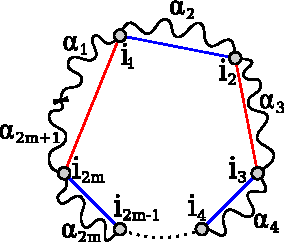
\includegraphics[scale=1.25]{kap7ChristofidesBew}
    \caption{Zu sehen ist die optimale Tour $\tau_{opt}$. $i_j$ sind die Knoten mit ungeradem Grad in $T$, $\alpha_k$ die Teilsequenzen von $\tau_{opt}$ zwischen diesen Knoten. Die blauen Kanten bilden ein Matching $M_1 = \{(i_1, i_2), (i_3, i_4), \ldots, (i_{2m-1}, i_{2m})\}$ zwischen den Knoten $i_j$, die roten ein alternatives Matching $M_2 = \{(i_2, i_3), (i_4, i_5), \ldots, (i_{2m}, i_1)\}$.}
    \label{kap7ChristofidesBew}
  \end{figure}
  
  In Abbildung \vref{kap7ChristofidesBew} sind auch zwei mögliche Matchings zwischen den Knoten ungeraden Grades eingezeichnet:
  \begin{align*}
    M_1 &= \{(i_1, i_2), (i_3, i_4), \ldots, (i_{2m-1}, i_{2m})\}\\
    M_2 &= \{(i_2, i_3), (i_4, i_5), \ldots, (i_{2m}, i_1)\}
  \end{align*}
   Das von der Christofides"=Heuristik gewählte Matching $M$ ist minimal, also gilt $c(M) \le c(M_1)$ und $c(M) \le c(M_2)$. Somit gilt $2 \cdot c(M) \le c(M_1) + c(M_2) \le c(\tau_{opt})$. Daraus folgt $c(M) \le \frac{1}{2} c(\tau_{opt})$.
   
   Wir können also die Kosten der gefundenen Tour $c(\tau)$ wie folgt abschätzen:
   \[ c(\tau) \le c(G) = c(T) + c(M) = c(T) + \frac{1}{2} \cdot c(\tau_{opt})\]
   Als wir bewiesen haben, dass die Baumheuristik $2$"=approximativ ist, haben wir $c(T) \le c(\tau_{opt})$ begründet, daher folgt
   \[ c(\tau) \le c(\tau_{opt}) + \frac{1}{2} \cdot c(\tau_{opt}) \]
\end{Bew}

\begin{Satz}
  \hspace{\parindent}Für kein $\alpha > 1$ gibt es einen $\alpha$"=approximativen Algorithmus polynomieller Laufzeit für \textsc{TSP}, es sei denn $\mathsf{P} = \mathsf{NP}$.
\end{Satz}

\begin{Bew}
  \hspace{\parindent}Angenommen es gäbe einen Approximationsalgorithmus für ein $\alpha > 1$ für \textsc{TSP}. Daraus könnten wir einen Polynomialzeit"=Algorithmus zur Lösung von \textsc{HC} konstruieren. Dazu geben wir an, wie wir aus einer Eingabe $G=(V,E)$ für \textsc{HC} eine Problemstellung für \textsc{TSP} konstruieren: Sei o.B.d.A. $V=\{1, \ldots, n\}$. Wir konstruieren die Problemstellung für \textsc{HC} wie folgt:
  \[ d_{ij} = \begin{cases} 1 & \text{falls } \{i,j\} \in E \\ 2 + \varepsilon n & \text{sonst}\end{cases} \qquad \text{mit } \varepsilon = \alpha -1 \]
  
  Wenden wir $A_\alpha$ auf diese Eingabe an, so gilt: $G$ hat Hamilton"=Kreis genau dann, wenn $A_\alpha$ eine Rundreise der Länge $n$ liefert.
  
  \glq$\Leftarrow$\grq: Aus einer Rundreise der Länge $n$ würde folgen, dass alle Kanten der Rundreise Kosten in Höhe von $1$ haben, das heißt sie wären alle Elemente aus $E$, es gäbe also einen Hamilton"=Kreis in $G$.
  
  \glq$\Rightarrow$\grq: Angenommen es gäbe einen Hamilton"=Kreis in $G$, dann gäbe es auch eine Rundreise der Länge $n$ in der \textsc{TSP}"=Instanz. Da $c(\tau_{opt}) = n$ gilt, liefert $A_{\alpha}$ eine Rundreise $\tau$ mit $c(\tau) \le \alpha n$. Jede Kante, die von $\tau$ genutzt wird muss aus $E$ stammen, $\tau$ hat also sogar die Länge $n$ und ist ein Hamilton"=Kreis. Angenommen das wäre nicht so, dann gäbe es eine Kante in $\tau$ mit einem Gewicht von $2 + \varepsilon n$. Dann wäre jedoch $c(\tau) \ge 2 + \varepsilon n + n - 1 = 2 + (\alpha - 1) n + n -1 = 1 + \alpha n$, was im Widerspruch dazu steht, dass $A_\alpha$ ein $\alpha$"=approximativer Algorithmus ist.
\end{Bew}

Also könnte man mit Hilfe von $A_{\alpha}$ \textsc{HC} (was ja \textsf{NP}"=vollständig ist) in polynomieller Zeit entscheiden. Dann wäre $\mathsf{P} = \mathsf{NP}$.

\textsf{NP}-schwere Optimierungsprobleme können bezüglich Approximation in verschiedene Schwierigkeitsgrade eingeteilt werden, falls $\mathsf{P} \neq \mathsf{NP}$. Solche unterschiedlich schwierigen Optimierungsprobleme können zum Beispiel welche sein, für die
\begin{itemize}
  \item keine Approximation mit einem Faktor $\alpha > 1$ in polynomieller Zeit möglich ist, wie zum Beispiel \textsc{TSP}.
  \item es ein $\alpha > 1$ (konstanter Faktor) gibt, so dass $\alpha$-Approximation in polynomieller Zeit möglich ist, wie zum Beispiel \textsc{$\varDelta$-TSP} oder auch Bin-Packing (aus der Übung).
  \item $\alpha$-Approximation in polynomieller Zeit für alle $\alpha > 1$ (beliebiger konstanter Faktor) möglich ist, wie zum Beispiel \textsc{Subset-Sum}.
\end{itemize}
%
%\subsection{Subset-Sum}
%Das Entscheidungsproblem \textsc{Subset-Sum} bekommt als Eingabe einige natürliche Zahlen $c_1, \ldots, c_n, k$. Das Entscheidungsproblem fragt ob es eine Teilmenge der Zahlen $c_1$ bis $c_n$ gibt, deren Summe $k$ ist. Das zugehörige Optimierungsproblem sucht die Teilmenge mit maximalem Gewicht $\le k$.
%
%\begin{Alg}[Approximationsalgorithmus für SUBSET-SUM]
%  \begin{algorithmic}[1]
%    \State $L_0 \mathrel{\mathop:}= (0)$
%    \For{$i = 1, 2, \ldots, n$}
%      \State $L_i \mathrel{\mathop:}= \mathtt{Mische}(L_{i-1}, L_{i-1} + c_i)$
%      \State entferne alle Elemente, die größer als $k$ sind aus $L_i$.
%    \EndFor
%    \State Gib größtes Element von $L_n$ aus.
%  \end{algorithmic}
%\end{Alg}
%
%$L_i$ ist die sortierte Liste aller Teilsummen von $c_1, \ldots, c_i$. Eine exakte Lösung für das Optimierungsproblem ist mit diesem Algorithmus berechenbar, braucht allerdings exponentielle Laufzeit.

% vorlesung 30 18.02.2011 (Fr)
%Es gibt (grob) 3 Klassen von \textsf{NP}-schweren Problemen:
%\begin{itemize}
%  \item Es ist keine Approximation in polynomieller Zeit möglich, es sei denn $\mathsf{P} = \mathsf{NP}$ (Bsp. \textsc{TSP})
%  \item Eine Approximation mit konstantem Faktor $\alpha$ ist in polynomieller Zeit möglich (Bsp. \textsc{$\varDelta$-TSP})
%  \item Es ist eine Approsimation mit beliebigem konstanten Faktor $1 + \varepsilon$ (oder $1 - \varepsilon$ je nachdem ob es ein Maximierungs- oder Minimierungsproblem ist) für jedes Feste $\varepsilon >0$ möglich in polynomieller Zeit (Bsp. \textsc{Subset-Sum}
%\end{itemize}

\subsection{Max3Sat}
\textsc{Max3Sat} ist ein Optimierungsproblem: gegeben ist eine Boolesche Formel in 3-KNF. Berechnet werden soll eine Belegung, die möglichst viele Klauseln wahr macht. Ist die Formel erfüllbar, so wird \textsc{Max3Sat} alle Klauseln wahr machen und so eine erfüllende Belegung finden. \textsc{Max3Sat} ist also, wie der Name schon sagt, ein Maximierungsproblem.

Ein $\frac{1}{2}$-approximativer Algorithmus, der in polynomieller Zeit arbeitet ist leicht zu finden. Setze dazu einmal alle Variablen auf $0$ und einmal alle Variablen auf $1$ und nimm die Belegung, die mehr Klauseln wahr macht. Eine Klausel die im ersten Schritt nicht wahr ist, ist im zweiten Schritt wahr und umgekehrt. Mindestens eine von beiden Belegungen muss die Mehrzahl der Klauseln wahr machen. Dadurch erhalten wir $\frac{1}{2}$"=Approximation.

Bekannt ist, dass \textsc{Max3Sat} sich nicht mit einem Faktor $>\frac{7}{8}$ in polynomieller Zeit approximieren lässt, es sei denn $\mathsf{P}=\mathsf{NP}$.

\subsection{Subset-Sum}
Gegeben sind einige natürliche Zahlen $c_1, \ldots, c_n, k$. Das Entscheidungsproblem fragt ob es eine Teilmenge der Zahlen $c_1$ bis $c_n$ gibt, deren Summe $k$ ist. Das zugehörige Optimierungsproblem sucht die Teilmenge mit maximalem Gewicht $\le k$. Für das Optimierungsproblem können wir folgenden Approximationsalgorithmus angeben:

\begin{Alg}
  \begin{algorithmic}[1]
    \State $L_0 \mathrel{\mathop:}= (0)$
    \For{$i:= 1, \ldots, n$}
      \State $L_i \mathrel{\mathop:}= \mathtt{Mische}(L_{i-1}, L_{i-1} + c_i)$ \Comment Wie bei Mergesort, elementenweise
      \State entferne alle Elemente $>k$ aus $L_i$
    \EndFor
    \State Gib das größte Element aus $L_n$ aus.
  \end{algorithmic}
\end{Alg}

$L_1 = (0, c_1)$, $L_2 = (0, c_1, c_2, c_1 + c_2)$ und so weiter. Das heißt $L_i$ ist die sortierte Liste aller Teilsummen von $c_1, \ldots, c_i$. Eine exakte Lösung für das Optimierungsproblem ist mit diesem Algorithmus berechenbar, braucht allerdings exponentielle Laufzeit, da $L_i$ exponentielle Größe hat. Wir wollen das dahingehend verbessern, dass man ein festes $\varepsilon > 0$ vorgibt und dann eine $(1 - \varepsilon)$"=Approximation des Problems erhält. Die Idee dazu ist jede Liste $L_i$ nach der Konstruktion wie folgt zu "`trimmen"'.

Unsere Methode \texttt{Trim} bekommt als Eingabe eine sortierte Liste $L = (y_1, \ldots, y_m)$ und ein $\delta >0$.

\begin{Alg}[$\mathtt{Trim}(L,\delta)$]
  \begin{algorithmic}[1]
    \State $L' = (y_1)$
    \For{$i \mathrel{\mathop:}= 2, \ldots, m$}
      \If{letztes Element von $L'$ $<(1-\delta) \cdot y_i$}
        \State hänge $y_i$ an $L'$ an.
      \EndIf
    \EndFor
    \State Gib $L'$ zurück
  \end{algorithmic}
\end{Alg}

\begin{figure}[htb]
  \centering
  \includegraphics[scale=1.5]{kap7Trimmen}
  \caption{Beim Trimmen, wird aus jedem Cluster ein Repräsentant genommen, in der Abbildung sind das $y_1, y_3, y_8, \ldots, y_m$. Zwischen den Repräsentanten gibt es einen Abstand von mindestens $1 - \delta$.}
\end{figure}

Der neue Approximations-Algorithmus, der \texttt{Trimm} nutzt, sieht dann aus wie folgt:
\begin{Alg}
  \begin{algorithmic}[1]
    \State $L_0 \mathrel{\mathop:}= (0)$
    \For{$i \mathrel{\mathop:}= 1, \ldots, n$}
      \State $L_i \mathrel{\mathop:}= \mathtt{Mische}(L_{i-1}, L_{i-1} + c_i)$ \Comment Wie bei Mergesort, elementenweise
      \State $L_i \mathrel{\mathop:}= \mathtt{Trim}(L_i, \frac{\varepsilon}{n})$
      \State entferne alle Elemente $>k$ aus $L_i$
    \EndFor
    \State Gib das größte Element aus $L_n$ aus.
  \end{algorithmic}
\end{Alg}

\begin{Beh}
  \hspace{\parindent}Der neue Approximations-Algorithmus für \textsc{Subset-Sum} liefert eine $(1-\varepsilon)$"=Approximation für das Problem und hat (für feste $\varepsilon$) polynomielle Laufzeit.
\end{Beh}

\begin{Bew}[Laufzeit des Approximationsalgorithmus]
  \hspace{\parindent}Betrachten wir zunächst die Laufzeit des Algorithmus und dann seine Qualität. Für die Laufzeit ist folgende Frage von großer Bedeutung: Wie lang kann $L_i$ nach dem Trimmen sein? Seien $s,t$ aufeinanderfolgende Elemente. Dann gilt %$\frac{t}{s} \ge \frac{1}{1-\frac{\varepsilon}{n}}$.
  \[ \frac{t}{s} \ge \frac{1}{1-\frac{\varepsilon}{n}} \]
  Betrachten wir nun $L_i = (0, s_1, \ldots, s_m)$ nachdem alle Elemente $>k$ entfernt wurden:
  \begin{align*}
    s_1 & \ge 1\\
    s_2 &\ge \frac{1}{1-\frac{\varepsilon}{n}} \\
    s_3 &\ge \frac{1}{(1- \frac{\varepsilon}{n})^2}\\
    & \ldots\\
    s_m &\ge \frac{1}{(1- \frac{\varepsilon}{n})^{m-1}} \le k
  \end{align*}
  Wir können das umformen:
  \begin{align*}
    \frac{1}{(1- \frac{\varepsilon}{n})^{m-1}} &\le k\\
    \ln \frac{1}{(1- \frac{\varepsilon}{n})^{m-1}} & \le \ln k\\
    \ln 1 - \ln ((1-\frac{\varepsilon}{n})^{m-1}) & \le \ln k\\
    -(m-1) \ln (1-\frac{\varepsilon}{n}) &\le \ln k\\
    m - 1 & \le \frac{\ln k}{-\ln (1-\frac{\varepsilon}{n})} \\
    m & \le \frac{\ln k}{-\ln (1-\frac{\varepsilon}{n})} + 1
  \end{align*}
  
  Es gilt $\ln (1- \frac{\varepsilon}{n}) \approx -\frac{\varepsilon}{n}$. Daher können wir $m$ (die Länge der Teillisten) auch wie folgt abschätzen:
  \[ m \le \frac{n \ln k}{\varepsilon} \]
  Die Listen bearbeiten wir $n$ mal. Wir kommen so auf eine Gesamtlaufzeit von $\mathcal{O}(\frac{n^2 \ln k}{\varepsilon})$, also $\mathcal{O}(n^2 \ln k)$ für festes $\varepsilon$. Das ist polynomiell in der Größe der Eingabe.
  
%  $-(m-1) \ln (1- \frac{\varepsilon}{n}) \ge \ln k$
%  
%  $\ln (1- \frac{\varepsilon}{n}) \approx -\frac{\varepsilon}{n}$
%  
%  Daher $-(m-1) \ln (1- \frac{\varepsilon}{n}) \ge \ln k$ insgesamt positiv.
%  
%  $m = \mathcal{O}(\frac{n \cdot \ln k}{\varepsilon})$
%  
%  Laufzeit insgesamt: $\mathcal{O}(\frac{n^2 \ln k}{\varepsilon})$ also $\mathcal{O}(n^2 \ln k)$ für festes $\varepsilon$, also polynomiell in Größe der Eingabe.
\end{Bew}

%  Qualität der Approximation
Nun kommen wir zur Qualität der Approximation. Sei $P_i$ wie folgt definiert.
\[ P_i = \{ \sum_{j \in S} c_j \mid S \subset \{ 1, \ldots, i \} \} \]
Dann gilt $L_i \subseteq P_i$. Unser Approximationsalgorithmus für \textsc{Subset-Sum} gibt $z \in L_n \subset P_n$ aus, es gilt also auch $z \in P_n$.

\begin{Beh}
  \hspace{\parindent} $z \ge (1- \varepsilon) \cdot s_{max}$, wobei $s_{max}$ die optimale Lösung für das Optimierungsproblem ist, also die größte Teilsumme $\le k$.
\end{Beh}

\begin{Bew}
  \hspace{\parindent}Sei $L'_i$ die Liste nach dem Trimmen von $L_i$. Zu jedem $s \in L_i$ existiert ein $s' \in L'_i$ mit $s \ge s' \ge (1 - \frac{\varepsilon}{n}) s$. In jedem Durchlauf ist der relative Fehler $\le (1- \frac{\varepsilon}{n})$. Insgesamt haben wir einen relativen Fehler von $(1- \frac{\varepsilon}{n})^n$. Das heißt $s_{max} \ge z \ge s_{max} (1- \frac{\varepsilon}{n})^n$.
  
%  Das heißt $s_{max} \ge z \ge s_{max} (1- \frac{\varepsilon}{n})^n$. $n$ im Nenner und im Exponenten sind zum Glück gegenläufig: $(1- \frac{\varepsilon}{n})^n$ wächst zwar exponentiell in $n$, nähert sich jedoch $1$ an. Im Übrigen $\lim\limits_{n \to \infty} (1 + \frac{x}{n})^n = e^x$
  
  Betrachten wir folgende Funktion: $f(x) = (1- \frac{\varepsilon}{x})^x$. Offensichtlich gilt $f(1) = 1 - \varepsilon$. Für alle $x \ge 1$ ist $f(x)$ streng monoton wachsend. Also gilt $(1- \frac{\varepsilon}{x})^x \ge (1-\varepsilon)$ für alle $x \ge 1$. Das heißt $s_{max} \ge z \ge s_{max} (1- \frac{\varepsilon}{n})^n \ge s_{max} (1-\varepsilon)$ für alle $n \ge 1$ gilt.
  
\end{Bew}

Ein fester Fehler $\varepsilon > 0$ kann also vorgegeben werden. Wir bekommen einen Polynom"=Zeit"=Algorithmus, der das Problem innerhalb von $1 - \varepsilon$ (bzw. ($1+ \varepsilon$)) approximiert. Ein solches $\varepsilon$-parametrisiertes Algorithmen-Schema heißt \textit{PTAS} (\textit{polynomial time approximation scheme}). Bei dem von uns angegeben Approximationsalgorithmus für \textsc{Subset-Sum} handelt es sich sogar um ein \textit{FPTAS}: \textit{fully PTAS}, da es auch polynomiell in $\frac{1}{\varepsilon}$ ist.

\section{alternative Ansätze}
Approximationsalgorithmen sind nur ein möglicher Ansatz für den Umgang mit Optimierungsproblemen. Alternativ kann man versuchen die Probleme doch exakt zu lösen, wobei dies nur in exponentieller Zeit oder mit guten Heuristiken für realistische Eingaben geht. Solche Heuristiken werden meist im Zusammenhang mit linearer Programmierung gefunden.

Einen anderen Ansatz bietet FPT (\textit{fixed parameter tractabilty}). Es gibt Probleme, die \textsf{NP}-schwer sind, für die es Algorithmen gibt, deren Laufzeit nicht nur von der Eingabelänge, sondern auch von einem Parameter $k$ abhängig ist. Ist $k$ eine Konstante, so lassen sich diese Probleme deutlich leichter lösen. Untersucht wird, ob sich diese Probleme auch mit variablem kleinen $k$ lösen lassen, wenn $k$ nicht in der Größenordnung von $n$ liegt. $f(k) \cdot p(n)$ wird derzeit untersucht, wobei $n$ die Eingabelänge, $p$ ein Polynom und $f$ eine berechenbare Funktion ist. Es gibt etliche \textsf{NP}-schwere Probleme, die sich für kleine $k$ lösen lassen, es gibt aber auch \textsf{NP}-schwere Probleme, bei denen dieser Ansatz nicht hilft. FPT dient somit auch dazu die Komplexität von \textsf{NP}-schweren Problemen besser zu differenzieren.

Das Gebiet dieser Vorlesung kann vertieft und fortgesetzt werden, durch den Besuch des Seminars über Algorithmen oder die Vorlesungen Höhere Algorithmik 2 und Algorithmische Geometrie.
